\documentclass[10pt,a4paper]{article}
\usepackage[T1]{fontenc}
\usepackage[english]{babel}
\usepackage{mathptmx}
% English language rules and explicit embedding for the PSNFSS Times family.
% Standard TeX Live/MiKTeX distributions provide these URW Type 1 fonts.
% The overrides also work when a site's pdftex.map omits Base-14 outlines.
\ifdefined\pdfmapline
  \pdfmapfile{+rsfs.map}
  \pdfmapline{=ptmr8r NimbusRomNo9L-Regu "TeXBase1Encoding ReEncodeFont" <8r.enc <utmr8a.pfb}
  \pdfmapline{=ptmb8r NimbusRomNo9L-Medi "TeXBase1Encoding ReEncodeFont" <8r.enc <utmb8a.pfb}
  \pdfmapline{=ptmri8r NimbusRomNo9L-ReguItal "TeXBase1Encoding ReEncodeFont" <8r.enc <utmri8a.pfb}
  \pdfmapline{=ptmbi8r NimbusRomNo9L-MediItal "TeXBase1Encoding ReEncodeFont" <8r.enc <utmbi8a.pfb}
  \pdfmapline{=psyr StandardSymL <usyr.pfb}
  \pdfmapline{=rpsyr StandardSymL <usyr.pfb}
  \pdfmapline{=pzcmi8r URWChanceryL-MediItal "TeXBase1Encoding ReEncodeFont" <8r.enc <uzcmi8a.pfb}
  \pdfmapline{=pcrr8r NimbusMonL-Regu "TeXBase1Encoding ReEncodeFont" <8r.enc <ucrr8a.pfb}
\fi
\renewcommand{\ttdefault}{pcr}
\ifdefined\pdfgentounicode\pdfgentounicode=1\fi
\ifdefined\pdfinclusioncopyfonts\pdfinclusioncopyfonts=1\fi
\AtBeginDocument{\selectlanguage{english}\lefthyphenmin=2\righthyphenmin=3}
\emergencystretch=1em

\newcommand{\aiplotnote}{Plotting code was developed with ChatGPT/Codex assistance.}
\usepackage[margin=22mm]{geometry}
\usepackage{amsmath,amssymb,booktabs,graphicx}
\usepackage[hidelinks]{hyperref}
\hypersetup{pdftitle={Supplement: Slowly Rotating Perfect-Fluid Spheres with an Adiabatic Gas Surface},pdfauthor={Jan Olsina}}
\newcommand{\dd}{\mathrm d}
\renewcommand{\thesection}{S\arabic{section}}
\renewcommand{\thetable}{S\arabic{table}}
\renewcommand{\thefigure}{S\arabic{figure}}
\title{Supplement to ``Slowly Rotating Perfect-Fluid Spheres\\with an Adiabatic Gas Surface''}
\author{Jan~Ol\v{s}ina\\[0.5ex]\small Independent Researcher, Prague, Czech Republic}\date{}
\begin{document}
\maketitle
\section{External rotational benchmarks}
All dimensionless quantities use the nonrotating mass and radius, with $G=c=1$:
$\mathcal C=M/R$, $\bar I=I/M^3$, and $\bar Q=-QM/J^2$; an oblate star has $Q<0$.
The matching solver is tested against the homogeneous-star table of Chandrasekhar and Miller~\cite{cm} and the $n=1$ polytropic curves of Yagi and Yunes~\cite{yy}. These are external model calculations, not universal-relation fits.

\begin{table}[h]
\centering\small
\caption{Homogeneous-star benchmark. Published values are converted from Table I of Ref.~\cite{cm}, using $\bar I=8(I/R_S^3)$ and $\bar Q=Q_{\rm table}/2$, with $R_S=2M$.}
\begin{tabular}{rrrrrrr}
\toprule
$\mathcal C$ & $\bar I_{\rm pub}$ & $\bar I_{\rm calc}$ & Difference (\%) & $\bar Q_{\rm pub}$ & $\bar Q_{\rm calc}$ & Difference (\%)\\
\midrule
0.25000000 & 8.392 & 8.39506760 & $+0.03655$ & 3.2625 & 3.26301980 & $+0.01593$\\
0.16666667 & 16.984 & 16.98235350 & $-0.00969$ & 7.8350 & 7.83589182 & $+0.01138$\\
0.10000000 & 43.896 & 43.89661657 & $+0.00140$ & 18.8650 & 18.86252015 & $-0.01315$\\
\bottomrule
\end{tabular}
\end{table}

For this test the background is the exact constant-density Schwarzschild interior. Its surface density is nonzero: no Love number or monopole mass correction is inferred from this test. The percentage agreement refers to the historical numerical table and does not imply agreement within half the last printed digit of every entry.

The polytropic benchmark uses $P=K\varepsilon^2$, as in Ref.~\cite{yy}. This differs from the thermodynamic rest-mass polytrope $P=K\rho_0^2$, $\varepsilon=\rho_0+P$, used in the main equal-compactness comparison. With $E=8\pi\varepsilon$ and a scale choice $\Pi=E^2$, the logarithmic enthalpy is $h=2\ln(1+E)$ and $c_s^2=2E$.

\begin{figure}[h]
\centering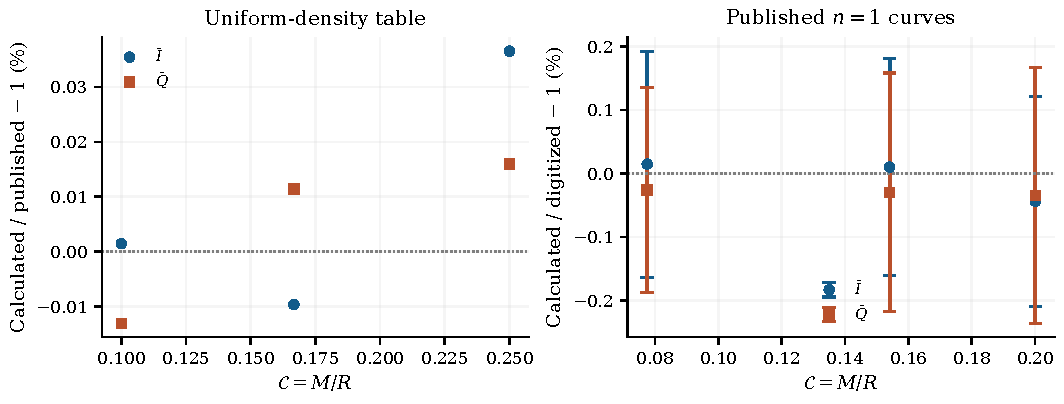
\includegraphics[width=\textwidth]{figures/external_benchmarks.pdf}
\caption{Relative differences from the published homogeneous-star table (left) and digitized $n=1$ curves (right). The right-hand error bars indicate a conservative graphical-resolution allowance, including both coordinate directions, not statistical errors or uncertainties assigned by the original authors. \aiplotnote}
\end{figure}

\clearpage
\section{Vector-figure extraction and thermodynamic limits}
The $n=1$ vertices come from the right-hand panels of Figs.~6 and 7 of Ref.~\cite{yy}, using the original source files \texttt{IbarC-PRD.eps} and \texttt{QbarC-PRD.eps}. Their $n=1$ line is orange and solid (\texttt{Color11}); the legend text precedes its associated line sample. Let $(x_v,y_v)$ denote the normalized drawing coordinates. The conversions are
\begin{align}
 \mathcal C&=0.004\,150^{x_v-0.15},\\
 \bar I&=3(1000/3)^{(y_v-0.15)/0.7},\qquad
 \bar Q=0.7(300/0.7)^{(y_v-0.15)/0.7}.
\end{align}
Ten checked axis ticks agree with these maps within $4.80\times10^{-5}$ in drawing coordinates. The three paired vertices are
\begin{align}
 (x_v,y_I,y_Q)={}&(0.7417,0.4838,0.5404),\nonumber\\
 &(0.8787,0.3318,0.4036),\quad(0.9308,0.2782,0.3384).
\end{align}
Allowing $\pm10^{-4}$ per coordinate accounts conservatively for rounding and calibration. The solver is evaluated at the central and shifted compactnesses; their response differences are combined with the vertical-coordinate allowance. This gives a graphical allowance of about $0.16$--$0.21\%$, compared with maximum observed differences of $0.044\%$ in $\bar I$ and $0.035\%$ in $\bar Q$. It is not an interval-certified bound on the underlying ODE solutions. The saved vertices and source hashes are included in the reproducibility archive.

\subsection*{Surface evaluation}
Write $s=r^2/R^2$, $z=\sqrt{1-s}$ and use $R=1$. The pressure integral
\begin{equation}
 \Pi(z)=\int_0^z t[E(t)+\Pi(t)]g(t)\,\dd t,
 \qquad E+\Pi=-4fa_j,
\end{equation}
avoids cancellation between order-$z^3$ terms when the pressure is order $z^5$. Similarly, $h(z)=\int_0^z t g(t)\,\dd t$ and $u_{\rm int}=\operatorname{expm1}(h)-\Theta$, where $\Theta=P/\rho_0$, resolve the vanishing internal energy. Differentiating $E+\Pi$ directly gives $E_z=(E+\Pi)_z-\Pi_z$ and a stable surface sound speed. Here quantities inside the integrals are composed with $s=1-t^2$.

\begin{figure}[h]
\centering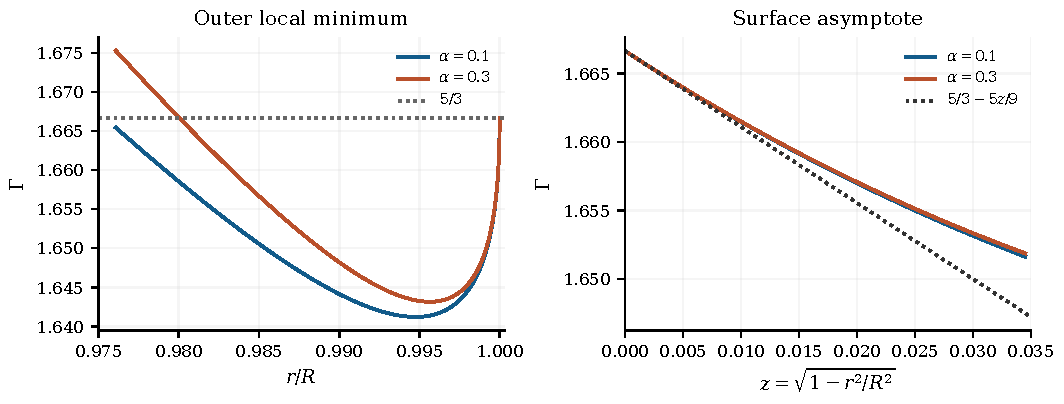
\includegraphics[width=\textwidth]{figures/gamma_surface_validation.pdf}
\caption{Resolved outer local minima of $\Gamma$ (left) and comparison with $\Gamma=5/3-5z/9+O(z^2)$ (right). The limiting value is reached from below. At $\alpha=0.3$ the outer minimum is local, since the central $\Gamma$ is smaller. \aiplotnote}
\end{figure}

\clearpage
\section{Thermodynamic convergence and pressure per particle}
The limiting relations are
\begin{equation}
 \Gamma=\frac53-\frac59z+O(z^2),\qquad
 \Theta=\frac{g_b}{5}z^2[1-z/3+O(z^2)],\qquad
 \frac{u_{\rm int}}{\Theta}\longrightarrow\frac32.
\end{equation}
Table~\ref{tab:limits} evaluates these relations at computed interior points. No flattening or smoothing toward an imposed surface value is used.
\begin{table}[h]
\centering
\caption{Surface convergence. The limiting entries in the last three columns are $-5/9$, $-1/3$ and $3/2$. Here $g_b=\mathcal C/(1-2\mathcal C)$.}
\label{tab:limits}
\begin{tabular}{rrrrr}
\toprule
$\alpha$ & $z$ & $(\Gamma-5/3)/z$ & $[5\Theta/(g_bz^2)-1]/z$ & $u_{\rm int}/\Theta$\\
\midrule
0.1 & $10^{-2}$ & $-0.518596$ & $-0.309150$ & 1.50795928\\
0.1 & $10^{-3}$ & $-0.551763$ & $-0.330885$ & 1.50082955\\
0.1 & $10^{-4}$ & $-0.555175$ & $-0.333088$ & 1.50008330\\
0.3 & $10^{-2}$ & $-0.516493$ & $-0.307191$ & 1.50793532\\
0.3 & $10^{-3}$ & $-0.551551$ & $-0.330689$ & 1.50082931\\
0.3 & $10^{-4}$ & $-0.555154$ & $-0.333069$ & 1.50008329\\
\bottomrule
\end{tabular}
\end{table}

At six interior radii, an independent five-point derivative check of
$\dd\ln\rho_0/\dd r=(\dd\varepsilon/\dd r)/(\varepsilon+P)$ has scaled residual below $1.7\times10^{-10}$. At three inner sample points, algebraic and hydrostatically integrated pressures agree within $6.4\times10^{-10}$ relatively. The metric and hydrostatic logarithmic enthalpies agree within $3\times10^{-13}$ absolutely at the checked points. These are floating-point diagnostics, not validated interval enclosures.

\begin{figure}[h]
\centering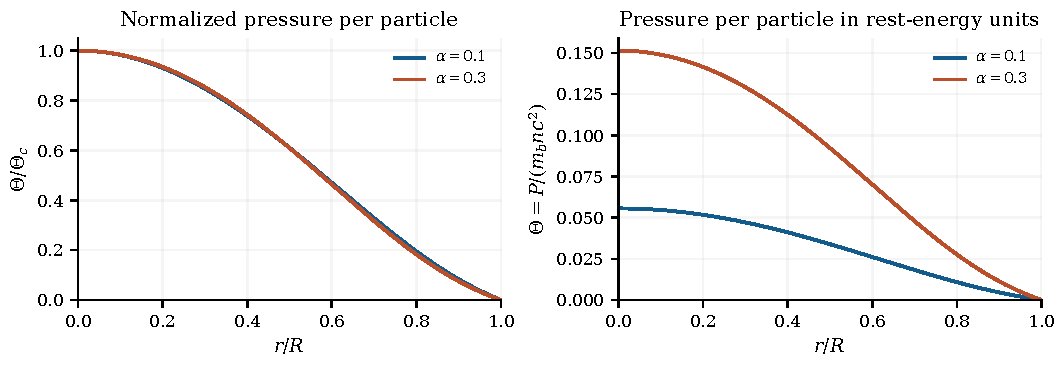
\includegraphics[width=\textwidth]{figures/pressure_per_particle.pdf}
\caption{Pressure per particle: normalized $\Theta/\Theta_c$ (left) and $\Theta=P/(m_bn c^2)$ (right). These curves are not a physical temperature profile. Only for a thermal ideal gas is $k_{\rm B}T=m_bc^2\Theta$; a cold degenerate gas can have the same leading surface law while $T=0$. The stiff core is outside either free-gas description. \aiplotnote}
\end{figure}

\begin{thebibliography}{9}
\bibitem{cm} S. Chandrasekhar and J.~C. Miller, \emph{Mon. Not. R. Astron. Soc.} \textbf{167}, 63--80 (1974), \href{https://doi.org/10.1093/mnras/167.1.63}{doi:10.1093/mnras/167.1.63}.
\bibitem{yy} K. Yagi and N. Yunes, \emph{Phys. Rev. D} \textbf{88}, 023009 (2013), \href{https://doi.org/10.1103/PhysRevD.88.023009}{doi:10.1103/PhysRevD.88.023009}; original figure sources from \href{https://arxiv.org/src/1303.1528}{arXiv:1303.1528}.
\end{thebibliography}
\end{document}
